\documentclass{book}
\usepackage{commeunjeustyle}

\newcommand{\FIK}{\mathcal{F}(I,\K  )}
\newcommand{\fn}{(f_n)_{n\in \N   }}
\newcommand{\Sfn}{\sum f_n}
\begin{document}
\chapter{Suites et séries de fonctions}

Dans le chapitre sur les séries numériques, nous avons étudié la série de Riemann, $\sum _{n\geq 1}{\frac {1}{n^{\alpha }}}$ dépendant du paramètre. Si $\alpha=1$, la série de Riemann s'appelle série harmonique et diverge. Si $\alpha=2$, la série de Riemann converge et est égale $\frac{\pi^2}{6}$.  On peut définir la fonction zêta de Riemann en considérant le paramètre $\alpha$ comme la variable, $x$, de la fonction, c'est à dire :
$$ \Fonction{\zeta}{]1,+\infty[}{\R }{x}{\sum _{n=1}^{\infty }\ {\frac {1}{n^{x}}}}.$$On a $\zeta(2)= \frac{\pi^2}{6}$. Ainsi définie comme la somme de la série, la fonction $\zeta$ est-elle continue, dérivable ? \\
La première partie de ce cours définira les notions de suites et séries de fonctions  ainsi que les différents modes de convergence. La fonction limite de la convergence simple sera définie comme la limite point à point. Ainsi définie, la fonction limite n'est pas garantie d'être continue, dérivable, etc. C'est pourquoi, nous définirons une convergence plus forte appelée convergence uniforme afin de garantir des propriétés de continuités, de dérivabilité, de permutation de la limite et de l'intégrale. Les théorèmes associés à ces  propriétés constitueront la dernière partie de ce cours. \\   
\textit{Notations} : 
\begin{itemize}
\item
  $I$ désigne un intervalle de $\R $ non vide et non réduit à un point
\item
  $\K  $ désigne $\R $ ou $\C    $
\item
  $\FIK$ désigne le $\K-$espace vectoriel des fonctions de $I$ dans $\K  $.
\end{itemize}

% -----------------------------------------------------------------------------

\section{Généralités}
\subsection{Définitions}

\begin{Definition}[Suite de fonctions]
On appelle \defi{suite de fonctions} toute suite $\fn$ à valeurs dans $\FIK$.
Autrement dit, une suite de fonctions est une suite $\fn$ dont les éléments sont des fonctions $f_n: I\to \K  $.
\end{Definition}
\begin{Exemple}\label{ex:1}Soit les suites $(f_n)_{n\in \N   }$, $(g_n)_{n\in \N^*   }$ et $(h_n)_{n\in \N   }$ définies par :
$$ \Fonction{f_n}{[0,1]}{\R }{x}{x^n},\quad \Fonction{g_n}{\R }{\R }{x}{\left(1+\frac x n\right)^n},\quad\Fonction{h_n}{\R ^+}{\R }{x}{x n^a e^{-nx}}.$$ 
\end{Exemple}

\begin{Definition}[Série de fonctions]
Soit $\fn$ une suite de fonctions de $I$ dans $\K  $.
On pose \[ \Fonction{S_n}{I}{\K  }{x}{\sum _{k=0}^n f_k(x)}.\]
On appelle \defi{série de fonctions} de $I$ dans $\K$ de terme général $f_n$, noté  $\sum _n f_n$, la suite des \defi{sommes partielles} $(S_n)_{n\in \N   }$.
\end{Definition}
\begin{Exemple}[Série entière]Les séries de la forme $\sum a_n x^n $  où $(a_n)_{n\in\N}$ est une suite réelle ou complexe. Par exemple, la série géométrique $\sum x^n$.
\end{Exemple}
\begin{Exemple}[Série trigonométrique]Les séries de la forme $\sum a_n  \cos (nx) $ et $\sum b_n  \sin (nx) $ où $(a_n)_{n\in\N}$ et $(a_n)_{n\in\N}$ suites réelles ou complexes.
\end{Exemple}

%% -----------------------------------------------------------------------------
\subsection{Modes de convergence}

% -----------------------------------------------------------------------------
\subsubsection{Convergence simple }
La convergence simple permet de définir une fonction comme limite d'une suite de fonctions ou d'une série de fonctions.

\begin{Definition}[Convergence simple  $\fn$]
Soit $\fn$ une suite de fonctions de $I$ dans $\K  $.\\
On dit que la suite de fonctions $\fn$ \defi{converge simplement} vers $f$ sur $I$ si  
\[  \forall x \in I, \text{ la suite numérique } (f_n(x))_{n\in \mathbb{N}} \text{ converge}, \] 
c'est à dire que $\lim\limits_{n \to \infty}f_n(x)$ existe dans $\K  $, pour tout $x\in I$. Dans ce cas, on peut définir la fonction:
$$
 \Fonction{f}{I}{\K  }{x}{\lim\limits_{n \to \infty}f_n(x)},$$
 appelée \defi{limite simple} sur $I$ de la suite $(f_n)_{n\in \N   }$.
\end{Definition} 

\begin{Methode}[Prouver la convergence simple]
        \begin{minipage}[c]{0.45\linewidth}{
Pour prouver que $\fn$ converge simplement vers $f$ sur $I$, il faut fixer la variable de  la fonction, \impo{Fixons $a\in I$},  et chercher à prouver que la \impo{suite numérique} $(f_n(a))_{n\in \N }$ converge vers $f(a)$. Il s'agit donc d'un problème de convergence d'une  suite numérique.\\
L'exemple ci dessous représente la convergence simple pour la suite $(f_n:x\to x^n)_{n\in \N }$. On fixe $a$ et on étudie la convergence de la suite $(f_n(a))_{n\in \N }$. 
}
\end{minipage}
    \begin{minipage}[c]{0.45\linewidth}{
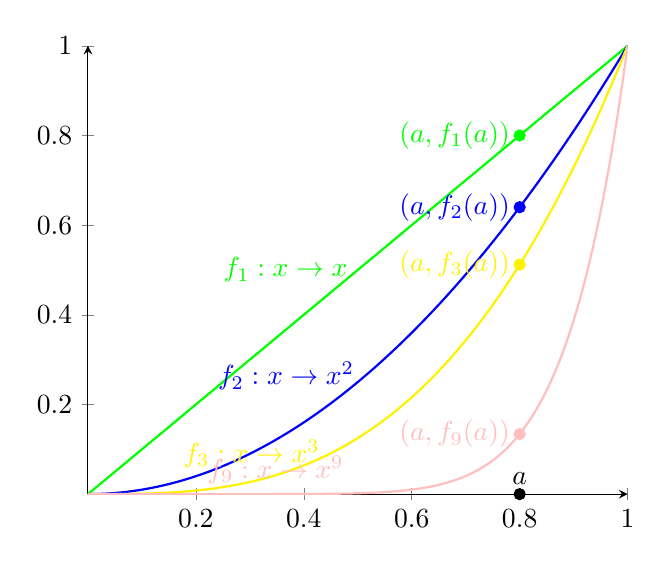
\begin{tikzpicture}
   \begin{axis}[
       axis y line = middle,
       axis x line = middle,
       samples     = 200,
       domain      = 0:1,
       xmin = 0, xmax = 1,
       ymin = 0, ymax = 1,
       unbounded coords=jump
     ]
     \addplot[black,mark=*] coordinates {(.8,0)}node[above] {$a$};
     \addplot[green, thick, mark=none] {x}node[pos=0.5, left] {$f_1:x\to x$};
     \addplot[green,mark=*] coordinates {(.8,.8)}node[left] {$(a,f_1(a))$}; 
     \addplot[blue, thick, mark=none] {x^2}node[pos=0.4, left] {$f_2:x\to x^2$};
     \addplot[blue,mark=*] coordinates {(.8,.64)}node[left] {$(a,f_2(a))$}; 
     \addplot[yellow, thick, mark=none] {x^3}node[pos=0.3,left] {$f_3:x\to x^3$};
     \addplot[yellow,mark=*] coordinates {(.8,.512)}node[left] {$(a,f_3(a))$};      
     \addplot[pink, thick, mark=none] {x^9}node[pos=0.2,above] {$f_9:x\to x^9$};
     \addplot[pink,mark=*] coordinates {(.8,.134)}node[left] {$(a,f_9(a))$};   
   \end{axis}
\end{tikzpicture}
}
    \end{minipage}
 \end{Methode}

\begin{Exemple}
Démontrons la convergence simples des suites de fonctions de l'exemple \ref{ex:1}.
\begin{enumerate}
\item 
Fixons $a\in [0,1]$.\\
\begin{itemize}
\item Si $a=1$, on a $a^n=1^n=1\xrightarrow[{n\to \infty}]{} 1$.
\item Si $a\neq 1$, la suite numérique $(a^n)_{n\in \mathbb{N}}$ est la suite géométrique de raison $q=a$. Comme $|a|<1$, la suite   converge vers 0. 
\end{itemize}
En conclusion, la suite de fonctions $(f_n)_{n\in \mathbb{N}}$ converge simplement vers la fonction limite $x \mapsto \begin{cases}0&{\text{si }}x\in[0,1[\\1&{\text{si } x=0}\end{cases} $ sur $[0,1]$.
\item 
Fixons $a\in \R $.
\begin{itemize}
\item Si $a=0$, on a $(1+\frac 0 n)^n=1\xrightarrow[{n\to \infty}]{} 1=e^0$.
\item Si $a\neq0$, on a :
$$
\begin{array}{rcl}
(1+\frac a n)^n &=& e^{n\ln (1+a/n)}\\
(1+\frac a n)^n &=& e^{n (a/n+o(1/n))}\\
(1+\frac a n)^n &=& e^{a+o(1)}\\
\end{array}
$$
Donc $\lim\limits_{n \to \infty}(1+\frac a n)^n=e^a$ car la fonction exponentielle est continue. 
\end{itemize}
En conclusion, la suite $(g_n)_{n\in \mathbb{N}}$ converge simplement vers la fonction $x \mapsto e^{x}$ sur $\R $.
\item 
Fixons $b\in \R ^+$.
\begin{itemize}
\item  Si $b=0$, on a $b n^a e^{-nb}=0\xrightarrow[{n\to \infty}]{} 0$.
\item Si $b\neq 0$, on a : $\lim\limits_{n \to \infty}b n^a e^{-nb}=0$ par croissance comparée.
%$$
%\begin{array}{rcl}
%n^a e^{-nb} &=& e^{a \ln n -nb}\\
%n^a e^{-nb} &=& e^{-nb(1-\frac{a \ln n}{nb})}\\
%n^a e^{-nb} &\underset{ \overset { n \rightarrow \infty } {} } {\sim}&e^{-nb}\xrightarrow[{n\to \infty}]{} 0.
%\end{array}
%$$ 
\end{itemize}
En conclusion,  la suite $(h_n)_{n\in \mathbb{N}}$ converge simplement vers la fonction nulle $x \mapsto 0$ sur $\R ^+$.
\end{enumerate}
\end{Exemple}


\begin{Remarque}  La suite de fonctions $(f_n)_{n\in \mathbb{N}}$ est une suite de fonctions continues sur $[0,1]$ et pourtant sa limite simple $x \mapsto \begin{cases}0&{\text{si }}x\in[0,1[\\1&{\text{si } x=0}\end{cases}$ n'est pas continue sur $[0,1]$.
\end{Remarque}

\begin{Definition}[Convergence simple  $\Sfn$]
On dit que la série $\Sfn$ \defi{converge simplement} sur $I$
si la suite de fonctions $(S_n)_{n\in \N   }$ converge simplement sur $I$.\\
Autrement dit, la série $\Sfn$ converge simplement sur $I$ si
\[  \forall  x\in I, \text{la série numérique } \sum _n f_n(x) \text{ converge.}  \]
Dans ce cas, la fonction :
$$
\Fonction{f}{I}{\K  }{x}{\sum_{n=0}^\infty f_n(x)}$$
 est appelé \defi{limite simple} sur $I$ de la série $\Sfn$.
\end{Definition}

\begin{Exemple}[Série géométrique] Soit la série de fonctions $\sum x^n$.\\
Fixons $a\in ]-1,1[$.\\
On a $\sum_{k=0}^n a^k= \frac{1-a^{n+1}}{1-a}\xrightarrow[{n\to \infty}]{}  \frac{1}{1-a}$ car $|a|<1$. \\
En conclusion,  la série  $\sum x^n$ converge simplement sur $]-1,1[$ vers la limite simple $x\mapsto \frac{1}{1-x}$.
\end{Exemple}

\begin{Proposition}[Unicité de la limite simple]
Soit $\fn$ une suite de fonctions de $I$ dans $\K  $.
Soit $f$ et $g$ deux fonctions de $I$ dans $\K  $.
Si $\fn$ converge simplement sur $I$ vers $f$ et vers $g$
alors $f = g$.
\end{Proposition}
\begin{Demonstration}
Supposons par l'absurde que $f\neq g$. Il existe donc $x\in I$ tel que  $f(x)\neq g(x).$ D'après l'hypothèse de convergence simple, en particulier, la suite numérique $(f_n(x))_{n\in\N}$ converge. Cela implique d'après l'unicité de la limite d'une suite numérique $f(x)=g(x)$. D'où la contradiction.  
\end{Demonstration}
%
%
\subsubsection{Convergence uniforme}
La convergence uniforme est une convergence plus forte que la convergence simple permettant de garantir des propriétés de continuité, de dérivabilité, etc,  sur la fonction limité définie à l'aide de la convergence simple. 

\begin{Definition}[Convergence uniforme $\fn$]
Soit $\fn$ une suite de fonctions de $I$ dans $\K  $, et soit $f \colon I \to\K  $.
On dit que la suite de fonctions $\fn$ \defi{converge uniformément} vers $f$ sur $I$ si 
\[ \forall  \epsilon>0 , \exists N\in \N , \forall  n\geq N ,\forall  x\in I, \left|f_n(x) - f(x)\right| \leq  \epsilon, \]
ou de façon équivalente, si la suite numérique $(\sup_{x\in I} \left|f_n(x) - f(x)\right|)_{n\in\mathbb{N}}$ converge vers 0, c'est à dire:
\[  \sup_{x\in I} \left|f_n(x) - f(x)\right|   \tend[n\to+\infty ]0.  \]
\end{Definition}

\begin{Proposition}
Si $\fn$ converge uniformément vers $f$, alors $\fn$ converge simplement vers $f$.
\end{Proposition}
\begin{Demonstration}
Fixons $a\in I$. On a$$ \left|f_n(a) - f(a)\right|\leq   \sup_{x\in I} \left|f_n(x) - f(x)\right|  \overbrace{\tend[n\to+\infty ]0.}^{\text{convergence uniforme}}$$
Donc la suite numérique $(f_n(a))_{n\in\N}$ converge vers $f(a)$. Donc  $\fn$ converge simplement vers $f$.
\end{Demonstration}
\begin{Methode}[Prouver la convergence uniforme]
On définit la limite simple, $f$, de la suite $\fn$ à l'aide de la convergence simple. Puis, on vérifie que le suite  $\fn$ converge uniformément vers cette limite $f$ car si la limite de convergence uniforme existe, elle est égale à celle de la convergence simple par 
\begin{enumerate}
\item\textit{ méthode 1} : une étude de fonction pour déterminer $\sup_{x\in I}\left|f_n(x) - f(x)\right|$
\item\textit{ méthode 2} :  une majoration $\sup_{x\in I}\left|f_n(x) - f(x)\right|$ par une quantité indépendante de $x$ et qui tend vers 0.
\end{enumerate}
\end{Methode}


\begin{Exemple}[Méthode 1] Soit $$\Fonction{h_n}{\R ^+}{\R ^+}{x}{n^a x e^{-nx} }.$$\\
\begin{itemize}
\item \textit{Conjecture :} l'animation geogebra \url{https://www.geogebra.org/graphing/bm5hggxd}, illustre la notion de convergence  pour   $a=0,5, a=1$ ou $a=1,5$. \\
Pour la \impo{convergence simple}, on fixe  $x$ (ici =0.3). On observe qu'à partir d'un certain rang de $n$, le point $x$  est à droite de la bosse quelque soit la valeur de $a$. Donc la suite numérique $(h_n(x))_{n\in\mathbb{N}}$ tend bien vers 0 quand $n$ tend vers $+\infty$ quelque soit les valeurs de $a$. La limite simple est la fonction nulle $h:x\to 0.$\\
Pour la \impo{convergence uniforme}, $x$ n'est plus fixé et appartient à l'intervalle $\R ^+$. $$\sup_{x\in \R ^+} \left|h_n(x) - h(x)\right|=\sup_{x\in \R ^+} \|h_n(x)\|$$ correspond à la hauteur de la bosse. On a convergence uniforme si et seulement si la hauteur tend vers $0$ quand quand $n$ tend vers $+\infty$. Pour $a=0,5$, la suite de fonctions $(h_n)_{n\in\mathbb{N}}$ converge uniformément car la bosse s'aplatit. En revanche, pour  $a=1$, la hauteur de la bosse reste constante et pour $a=1,5$, la hauteur tend vers  $+\infty$  quand $n$ tend vers $+\infty$. La suite de fonctions $(h_n)_{n\in\mathbb{N}}$ ne converge pas uniformément pour ces deux dernières valeurs. On conjecture que la convergence est uniforme si et seulement si $a<1$.
\item \textit{Preuve :} pour étudier la convergence uniforme de la suite de fonctions $(h_n)$,  on étudie la suite numérique  $\left(\sup_{x\in  \R ^+} \|h_n(x)\| \right)_{n\in\N}$. Comme $h_n$ est une fonction dérivable, on étudie le signe de sa dérivée. Soit $x\in  \R ^+$. 
$${h'}_n(x)=n^a(e^{-nx}-nxe^{-nx})=n^ae^{-nx}(1-n).$$ D'où ${h'}_n(x)\geq 0 \Leftrightarrow  x\leq \frac 1 n.$  
\begin{center}
\begin{tikzpicture}
   \tkzTabInit{$x$ / 1 , Signe de $h'_n(x)$ / 1, Variations $h_n$ / 1.5}{$0$, $\dfrac{1}{n}$, $+\infty$}
   \tkzTabLine{, +, z, -, }
   \tkzTabVar{-/ 0, +/ $h_n\left(\dfrac{1}{n}\right)$, -/ 0}
\end{tikzpicture}
\end{center}
$|h_n|$ atteint son maximum en $1/n$, d'où $$\sup_{x\in  \R ^+} \left|h_n(x) \right|=h_n(1/n)=n^{a-1}e^{-1}\xrightarrow[{n\to \infty}]{}\begin{cases} 0 &\text{ si }  a<1\\e^{-1} &\text{ si }  a=1\\+\infty &\text{ si }  a>1 \end{cases}.$$ Donc $(h_n)_{n\in\mathbb{N}}$ converge uniformément si et seulement si   $a<1.$
\end{itemize}
\end{Exemple}

\begin{Exemple}[Méthode 2]
Soit la suite de fonctions $(f_n:x\mapsto x^n)_{n\in \mathbb{N}}$ convergeant simplement vers la fonction nulle $x\mapsto 0$ sur $[0,a]$ avec $0<a<1$. On a :
$$\forall n\in \N, \forall x\in[0,a]:\quad |x^n|\leq a^n$$ c'est à dire :
$$ \forall n\in \N, \sup_{x\in[0,a]}|x^n|\leq a^n.$$
Comme $a^n\tend[n\to+\infty]0$, on déduit que $\sup_{x\in[0,a]}|x^n| \tend[n\to+\infty]0$ par théorème de comparaison. \\
En conclusion, la suite de fonctions $(x\mapsto x^n)_{n\in \mathbb{N}}$ converge uniformément vers la fonction nulle $x\mapsto 0$ sur $[0,a]$ .
\end{Exemple}


\begin{Definition}[Convergence uniforme $\Sfn$]
On dit que la série $\Sfn$ \defi{converge uniformément} sur $I$ si  la suite de fonction $(S_n)_{n\in \N   }$ converge uniformément sur $I$.
\end{Definition}
\begin{Proposition}[Critère du reste]
Soit $\Sfn$ une série de fonction qui converge simplement vers $f$ sur $I$.\\
Cette série converge uniformément vers $f$ sur $I$ si et seulement si
la suite de fonctions $(R_n)$ converge uniformément vers $0$ sur $I$
où \[ R_n(x) = \sum _{k>n} f_k(x). \]
Ainsi, montrer que $\Sfn$ converge uniformément sur $I$ revient à montrer
l'existence d'une suite réelle $(\epsilon_n)_{n\in \N   }$ telle que:
  \begin{itemize}
  \item
    $\forall  n\in \N   $, $\forall  x\in I$, $\left|R_n(x)\right| \leq \epsilon_n$;
  \item
    la suite numérique $(\epsilon_n)$ tend vers $0$.
  \end{itemize}
\end{Proposition}
\begin{Demonstration}
Cette égalité prouve l'équivalence :
 $$ \sup_{x\in I}\left|\sum_{k=0}^{n} f_n(x) - f(x)\right| = \sup_{x\in I}\left|\sum_{k=0}^{n} f_n(x) - \sum_{k=0}^{+\infty}f_n(x)\right|=\sup_{x\in I}\left|\sum_{k=n+1}^{\infty} f_n(x)\right|  $$ 
\end{Demonstration}

\begin{Exemple} Soit la série de fonctions $\sum \frac{(-1)^n}{x+n}$.\\
La série de fonctions converge simplement sur $\R^+$, car à $x\in\R^+ $ fixé, la série numérique $\sum \frac{(-1)^n}{x+n}$ respecte le critère de convergence des séries alternées : $(\frac{1}{x+n})_{n\in\mathbb{N}}$ est une suite décroissante de limite 0. Pour la convergence uniforme, la valeur absolue du reste d'une série alternée est majorée par celle de son premier terme:
$$\forall  x\in \R ^+,\left|R_n(x)\right| \leq  \left|\frac{1}{x+(n+1)}\right|\leq \frac{1}{n+1}\xrightarrow[{n\to \infty}]{} 0.$$
\end{Exemple}
% 
% -----------------------------------------------------------------------------
\subsubsection{Convergence normale}

Uniquement pour les séries de fonctions, la convergence normale est une convergence plus forte que la convergence uniforme. Elle est avant tout un outil pour démontrer la convergence uniforme car démontrer qu'une série converge normalement est souvent évident.  

\begin{Definition}[Convergence normale $\Sfn$]
Soit $\Sfn$ une série de fonctions bornées de $I$ dans $\K  $.
On dit que la série de fonctions $\Sfn$ \defi{converge normalement} sur $I$
si  la série numérique
de terme général $u_n = \sup_{x\in I} \left|f_n(x)\right|$ converge.
\end{Definition}
\begin{Proposition}
Soit $\Sfn$ une série de fonctions de $I$ dans $\K  $.
Montrer que la série converge normalement sur $I$ revient à
montrer l'existence d'une suite réelle $(\alpha_n)_{n\in \N   }$ telle que:
  \begin{itemize}
  \item
    $\forall  n\in \N   $, $\forall  x\in I$, $\left|f_n(x)\right|\leq \alpha_n$;
  \item
    la série numérique $\sum \alpha_n$ converge.
  \end{itemize}
\end{Proposition}
\begin{Demonstration}
La série numérique $ \sum \sup_{x\in I} \left|f_n(x)\right|$ est une série à termes positifs dont le terme général est bornée par $\alpha_n$. Comme la sérié numérique $\sum \alpha_n$ converge, la série numérique $ \sum \sup_{x\in I} \left|f_n(x)\right|$ par règle de comparaison.
\end{Demonstration}


\begin{Proposition}
La convergence normale entraîne la convergence uniforme (qui entraîne la convergence simple).
\end{Proposition}
\begin{Demonstration}
Soit $n<N$.
$$\forall  x\in I:\quad  \left|\sum_{k=n+1}^{N} f_n(x)\right|\leq  \sum_{k=n+1}^{N} \left|f_n(x)\right|   \leq  \sum_{k=n+1}^{N} \sup_{x\in I} \left|f_n(x)\right|  \overbrace{\leq}^{\text{Série à termes positifs}} \sum_{k=n+1}^{+\infty} \sup_{x\in I} \left|f_n(x)\right|. $$ 
Par passage à la limite, l'inégalité devient :
 $$\forall  x\in I:\quad  \left|\sum_{k=n+1}^{+\infty} f_n(x)\right|\leq  \sum_{k=n+1}^{+\infty} \sup_{x\in I} \left|f_n(x)\right| . $$ 
Comme la série converge normalement, la série $\sum \sup_{x\in I} \left|f_n(x)\right|$ converge et son reste $(\sum_{k=n+1}^{+\infty}  \sup_{x\in I} \left|f_n(x)\right| )_{n\in\N}$ converge vers 0. Ainsi la série $\Sfn$ converge absolument par le critère des restes. 
\end{Demonstration}
\begin{Exemple}Soit la série de fonctions $\sum \frac{\sin(nx)}{n^2}$.\\
On a :
$$\forall n\in\N^* :\quad \left|\frac{\sin(nx)}{n^2}\right|\leq \frac{1}{n^2}.$$
Comme la série de Riemann $\sum \frac{1}{n^2}$ est convergente,  la série de fonctions $\sum \frac{\sin(nx)}{n^2}$ converge normalement donc uniformément.
\end{Exemple}
\begin{Remarque}La convergence uniforme n'implique pas la convergence normale. La série de fonctions $\sum \frac{(-1)^n}{x+n}$ converge uniformément sur $\mathbb{R}^+$ mais pas normalement. On a$$ \forall  n\in \N   , \sup_{x\in \mathbb{R}^+}\left| \frac{(-1)^n}{x+n}\right|=\frac{1}{n}.$$ La série harmonique $\sum \frac{1}{n}$ est divergente.
\end{Remarque}

\section{Régularité de la limite d'une suite/série de fonctions}

\subsection{Continuité}\label{sec:cont}
\begin{Theoreme}[Théorème de la permutation des limites]
Soit $\fn$ une suite de fonctions de $I$ dans $\K  $.
On suppose que:
\begin{itemize}
\item
  $a$ est un point ou une extrémité de $I$ (éventuellement $±\infty$);
\item
  pour tout $n\in \N   $, $\lim\limits_{x\to a} f_n(x) = l_n$ existe et est finie;
\item
  $\fn$ converge uniformément vers $f$ sur $I$.
\end{itemize}
Alors:
\begin{itemize}
\item
  la suite $(l_n)_{n\in \N   }$ converge. Notons $l$ sa limite.
\item
  $\lim\limits_{x\to a} f(x) = l$, c'est à dire
  \[ 
      \lim_{x\to a} \; \lim_\ninf \; f_n(x) = \lim_\ninf \; \lim_{x\to a} \; f_n(x).
   \]
\end{itemize}
\end{Theoreme}
%\begin{Demonstration}[Hors programme (utilisation du critère de Cauchy)]
%On a :
%\begin{itemize}
%\item \textit{$(l_n)_{n\in\N}$ suite de Cauchy :} Soit $ \varepsilon >0$. \\
%Comme $\fn$ converge uniformément vers $f$, il existe $N$ tel que,
%$$\forall n>N:\quad \sup_{x\in I } \vert f_{n}(x)-f(x)\vert\leq\varepsilon.$$ 
%Soit $x\in I$, $n>N$ et $k\in \N$.
%$$\vert f_{n+k}(x)-f_n(x)\vert \leq \vert f_{n+k}(x)-f(x) \vert + \vert f_{n}(x)-f(x) \vert\leq \sup_{x\in I } \vert f_{n+k}(x)-f(x)\vert +\sup_{x\in I } \vert f_{n}(x)-f(x)\vert\leq 2\varepsilon $$ 
%Dans cette inégalité, prenons la limite quand $ x$ tend vers $ a$, 
%$$\displaystyle \vert l_{n+k}-l_n\vert\leqslant 2\varepsilon.$$
%En conclusion, $(l_n)_{n\in\N}$ est une suite de Cauchy. Comme $\K$ est complet, $(l_n)_{n\in\N}$ converge vers une limite $l$.
%  \item \textit{$\lim\limits_{x\to a} f(x) = l$ : } Soit $ \varepsilon >0$. \\
%  $$\vert f(x)-l\vert \leq  \vert f(x)- l\vert $$ 
%  
%\end{itemize}
%\end{Demonstration}

\begin{Theoreme}[Théorème de permutation limite-somme]
Soit $\Sfn$ une série de fonctions de $I$ dans $\K  $.
On suppose que:
\begin{itemize}
\item
  $a$ est une extrémité de $I$ (éventuellement $±\infty $);
\item
  pour tout $n\in \N   $, $\lim\limits_{x\to a} f_n(x) = l_n$ existe et est finie;
\item
  $\Sfn$ converge uniformément vers $f$ sur $I$.
\end{itemize}
Alors:
\begin{itemize}
\item
  la série numérique $\sum _n l_n$ est absolument convergente;
\item
  $f$ admet une limite en $a$;
\item
  $\lim_a f = \sum _{n=0}^{+\infty } l_n$, c'est à dire
  \[  \lim_{x \to a} \sum _{n=0}^{+\infty } f_n(x) = \sum _{n=0}^{+\infty } \lim_{x \to a} f_n(x).  \]
\end{itemize}
\end{Theoreme}

\begin{Exemple} La série $\sum\frac {1}{n^{x}}$ converge uniformément sur $[a,+\infty[$ avec $a>1$. On a :
$$\lim_{x\to \infty }\zeta(x)=\lim_{x\to \infty } \sum _{k=1}^{\infty} \frac {1}{k^{x}} = \lim_{x\to \infty }\lim_{n\to \infty } \sum _{k=1}^{n } \frac {1}{k^{x}}= \lim_{n\to \infty } \lim_{x\to \infty } \sum _{k=1}^{n } \frac {1}{k^{x}}  = \lim_{n\to \infty }  \sum _{k=1}^{n }\lim_{x\to \infty } \frac {1}{k^{x}}  =\lim_{n\to \infty } (1+0+\dots +0) =1.
$$
\end{Exemple}

\begin{Theoreme}[Théorème de continuité de la limite]
La limite uniforme d'une suite de fonctions continue est elle-même continue.\\
Plus précisément, si
\begin{itemize}
\item
  pour tout $n\in \N   $, $f_n$ est continue sur $I$,
\item
  $\fn$ converge uniformément vers $f$.
\end{itemize}
Alors $f$ est continue sur $I$.
\end{Theoreme}
\begin{Demonstration}
Ce théorème est un corollaire du théorème de la double limite. Soit $a\in I$. On a :
$$\lim_{x\to a} f(x)=\lim_{x\to a}\lim_\ninf \; f_n(x) \underset{\text{th double limite}}{=}\lim_\ninf \lim_{x\to a} \; f_n(x)\underset{f_n \text{ continue}}{=}\lim_\ninf f_n(a)= f(a).  $$
\end{Demonstration}
%
\begin{Remarque}
Par contraposition, le théorème précédent permet, dans certains exemples, de montrer la non-convergence uniforme. \\ 
Par exemple, la suite de fonctions $(x\mapsto x^n)_{n\in \mathbb{N}}$ converge simplement sur $[0,1]$ vers  $x \mapsto \begin{cases}0&{\text{si }}x\in[0,1[\\1&{\text{si } x=0}\end{cases}$ mais ne converge pas uniformément  sur $[0,1]$ car chaque $x\mapsto x^n$ est continue et sa limite simple ne l'est pas.
\end{Remarque}
%% -----------------------------------------------------------------------------
\begin{Theoreme}[Théorème de continuité de la somme]
Soit $\Sfn$ une série de fonctions de $I$ dans $\K  $.
On suppose que:
\begin{itemize}
\item
  pour tout $n\in \N   $, $f_n$ est continue sur $I$;
\item
  $\Sfn$ converge uniformément sur $I$.
\end{itemize}
Alors la somme $f = \sum _{n=0}^{+\infty } f_n$ est une fonction définie et continue sur $I$.
\end{Theoreme}
\begin{Remarque}La notion de continuité est une notions \impo{locale}. Cela signifie que pour montrer qu'une fonction $f$ est continue sur un intervalle $I$, il faut montrer que $f$ est continue en tout point $a$ de l'intervalle.\\
Ainsi, dans les théorèmes sur la continuité , on peut remplacer l'hypothèse de convergence uniforme sur $I$ par la convergence uniforme sur tout segment $K$ inclus dans $I$.\\
Par exemple, la série $\sum\frac {1}{n^{x}}$ ne converge pas uniformément sur $]1,+\infty[$ mais converge normalement donc uniformément sur  $[a,+\infty[$, pour tout $a>1$. Donc, la fonction limite,   $\zeta$ est continue $[a,+\infty[$, pour tout $a>1$ donc continue sur  $]1,+\infty[$.
\end{Remarque}
\subsection{Permutation avec une intégrale}\label{sec:perm-int}

\begin{Theoreme}[Théorème de permutation limite/intégrale]
Soit $\fn$ une suite de fonctions de $I$ dans $\K  $.
On suppose que:
\begin{itemize}
\item
  pour tout $n\in \N   $, $f_n$ est continue sur le segment $[a,b]$;
\item
  $\fn$ converge uniformément vers $f$ sur $[a,b]$.
\end{itemize}
Alors $f$ est continue (donc intégrable) sur $[a,b]$ et
\[  \lim_\ninf \int_a^b f_n(t)dt = \int_a^b \lim_\ninf f_n(t)dt = \int_a^b f(t)dt. \]
\end{Theoreme}
\begin{Demonstration}
$$\begin{aligned}
\left|\int_a^b f_n(t)dt -\int_a^b f(t)dt\right|=&\left|\int_a^b (f_n(t)-f(t))dt\right|\\
\leq&\int_a^b\left|f_n(t)-f(t)\right|dt\\
\leq &\sup_{x\in[a,b]}\left|f_n(t)-f(t)\right|\int_a^b dt=(b-a) \sup_{x\in[a,b]}\left|f_n(t)-f(t)\right|  \tend[n\to+\infty ]0.
\end{aligned}$$ 
\end{Demonstration}

\begin{Remarque}
Si il n'y pas convergence uniforme, on ne peut pas permuter en générale limite et intégrale. \\
Par exemple, on observe dans cette animation géogébra \url{https://www.geogebra.org/graphing/qwwbjxgv},
 \begin{center}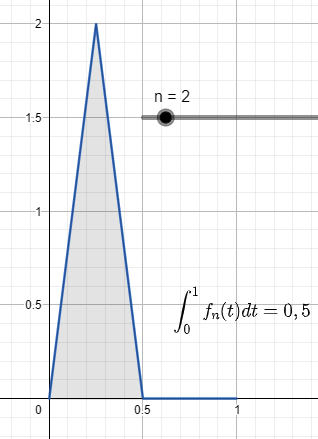
\includegraphics[width=3cm]{contre_exemple_limite_integrale.png}\end{center} que la suite de fonctions $\fn$ converge simplement vers la fonction nulle sur $[0,1]$. L'intégrale de la fonction nulle sur $[0,1]$ est $0$. Comme l'intégrale de chaque fonctions $f_n$ est $\frac 1 2$, la limite des intégrales est $\frac 1 2$. L'égalité n'est donc pas vérifiée car $$ \lim_\ninf \int_0^1 f_n(t)dt =  \lim_\ninf \frac 1 2 = \frac 1 2 \neq 0  = \int_0^1 0dt= \int_0^1 \lim_\ninf f_n(t)dt.$$
On peut vérifier que la suite de fonctions $\fn$ définie par :
$$\forall n \in \mathbb{N}^* :\quad  \Fonction{f_n}{[0,1]}{\mathbb{R}}{x}{\begin{cases}2n^2x&\text{ si } 0\leq x < \frac{1}{2n}\\2n-2n^2x&\text{ si } \frac{1}{2n}\leq x < \frac{1}{n}  \\0&\text{ si } \frac{1}{n}\leq x \leq 0 \end{cases}}$$ converge et simplement vers la fonction nulle et que  $\int_0^1 f_n(t)dt = \frac 1 2$. 
\end{Remarque}
\begin{Theoreme}[Théorème de permutation somme/intégrale]
Soit $\Sfn$ une série de fonctions de $[a,b]$ dans $\K  $.
On suppose que:
\begin{itemize}
\item
  pour tout $n\in \N   $, $f_n$ est continue sur le segment $[a,b]$
\item
  la série de fonctions $\sum _n f_n$ converge uniformément sur $[a,b]$ vers $f$
\end{itemize}
Alors $f$ est continue sur $[a,b]$ (donc intégrable) et
\[  \sum _{n=0}^{+\infty } \int_a^b f_n(t)dt = \int_a^b \sum _{n=0}^{+\infty } f_n(t)dt= \int_a^b f(t)dt.   \]
\end{Theoreme}

\begin{Demonstration}
Le théorème de permutation de limite/intégrale  sur les suites nous donne :
\[ \lim_{n\to +\infty}\int_a^b S_n(t)dt =\int_a^b\lim_{n\to +\infty} S_n(t) dt \]
En substituant dans cette égalité  
$$\lim_{n\to +\infty}\int_a^b S_n(t)dt=\lim_{n\to +\infty}\int_a^b\sum_{k=0}^n f_n(t)dt\overbrace{=}^{\text{somme finie}}\lim_{n\to +\infty}\sum_{k=0}^n \int_a^b f_n(t)dt=\sum _{k=0}^{+\infty } \int_a^b f_k(t)dt$$
et 
$$\int_a^b\lim_{n\to +\infty} S_n(t) dt =\int_a^b\lim_{n\to +\infty} \sum_{k=0}^n f_n(t) dt = \int_a^b \sum _{k=0}^{+\infty } f_k(t)dt$$
on obtient le résultat. 
\end{Demonstration}



\begin{Exemple}[Série géométrique] La série $\sum x^n$ converge uniformément vers la fonction $x\mapsto \frac{1}{1-x}$ sur $[0,a]$ avec $0<a<1$.  Comme
$$ \forall x \in [0,1[, \int_0^x \sum _{n=0}^{+\infty } t^n dt \overbrace{=}^{Th} \sum _{n=0}^{+\infty } \int_0^x t^n dt = \sum _{n=0}^{+\infty } \frac{x^{n+1}}{n+1},$$
et
$$\forall x \in [0,1[, \int_0^x \frac{1}{1-t} dt = -\ln(1-x),$$
Par intégration de  
$$\forall x \in [0,1[,   \frac{1}{1-x} = \sum _{n=0}^{+\infty } x^n,$$
on obtient le développement en série entière de la fonction $x:\mapsto  \ln(1-x)$ :
$$\forall x \in [0,1[,-\ln(1-x)=  \sum _{n=0}^{+\infty } \frac{x^{n+1}}{n+1}.$$
\end{Exemple}

\subsection{Dérivabilité}\label{sec:deriv}
%
\begin{Theoreme}[Dérivation de la limite]
Soit $\fn$ une suite de fonctions de $I$ dans $\K  $.
On suppose que:
\begin{itemize}
\item
  pour tout $n\in \N   $, $f_n$ est de classe $C^1$ sur $I$;
\item
  $\fn$ converge simplement vers $f$ sur $I$;
\item
  $(f'_n)_{n\in\N}$ converge uniformément vers $g$ sur $I$.
\end{itemize}
Alors:
\begin{itemize}
\item
  $f$ est de classe $C^1$ sur $I$;
\item
  $f' = g$ c'est à dire:
$$\forall x \in I:\quad  \left(\lim_\ninf f_n(x) \right)'=\lim_\ninf f'_n(x)$$
  
  
\end{itemize}
\end{Theoreme}
\begin{Theoreme}[Dérivation de la somme]
Soit $\Sfn$ une série de fonctions de $I$ dans $\K  $. On suppose que:
\begin{itemize}
\item
  pour tout $n\in \N   $, $f_n$ est de classe $C^1$ sur $I$
\item
  $\sum _n f_n$ converge simplement sur $I$ vers $f$
\item
  $\sum _n f'_n$ converge uniformément sur $I$
\end{itemize}

Alors $f$ est de classe $C^1$ sur $I$ et
\[ \forall  x\in I :\quad \left(\sum _{n=0}^{+\infty } f_n(x)\right)' = \sum _{n=0}^{+\infty } f'_n(x). \]
\end{Theoreme}
%
\begin{Exemple} La série $\sum x^n$ converge simplement vers la fonction $x\mapsto \frac{1}{1-x}$ sur $[-a,a]$ avec $0<a<1$.
La série dérivée $\sum n x^{n-1}$ converge uniformément sur $[0,a]$ avec $0<a<1$ car elle converge normalement sur  $[-a,a]$. En effet,
$$ \forall n\in \mathbb{N}^*, \sup_{x\in[-a,a]} |n x^{n-1}|=n a^{n-1},$$ 
or la série $\sum n a^{n-1}$ converge en utilisant le critère de d'Alembert ($\lim \frac{(n+1)a^{n}}{n a^{n-1}}=a<1$). Donc la série  $\sum n x^{n-1}$ converge uniformément vers $f':x\mapsto \left(\frac{1}{1-x}\right)'=\frac{1}{(1-x)^2}$ sur $[-a,a]$. 
\end{Exemple}
%
%% -----------------------------------------------------------------------------
\subsection{Généralisation}\label{sec:deriv2}

\begin{Theoreme}[Dérivation de la limite]
Soit $\fn$ une suite de fonctions de $I$ dans $\K  $.
On suppose que:
\begin{itemize}
\item
  pour tout $n\in \N   $, $f_n$ est de classe $C^p$ sur $I$, $p>1$;
\item
  pour tout $k\in \{0,\dots, p-1\}$,
  la suite $(f^{(k)}_n)_{n\in\N}$ converge simplement vers $g_k$ sur $I$;
\item
  la suite $(f^{(p)}_n)_{n\in\N}$ converge uniformément vers $g_p$ sur $I$.
  \end{itemize}
Alors:
\begin{itemize}
\item
  $f=g_0$ est de classe $C^p$;
\item
 $\forall  k\in \{0,\dots, p\}$, $f^{(k)} = g_k$.
\end{itemize}
\end{Theoreme}
\begin{Theoreme}[Théorème de dérivation de la somme]
Soit $\Sfn$ une série de fonctions de $I$ dans $\K  $.
On suppose que:
\begin{itemize}
\item
  pour tout $n\in \N   $, $f_n$ est de classe $C^p$, $p>1$
\item
  pour tout $k\in \{0,\dots, p-1\}$, $\sum _n f_n^{(k)}$ converge simplement sur $I$
\item
  $f$ est la somme de la série $\Sfn$, c.-à-d. $f =\sum _{n=0}^{+\infty } f_n$
\item
  $\sum _n f_n^{(p)}$ converge uniformément sur $I$
\end{itemize}
Alors $f$ est de classe $C^p$ sur $I$ et
\[ \forall  k\in  \{0,\dots, p\}, \forall  x\in I,\quad f^{(k)}(x) = \sum _{n=0}^{+\infty } f^{(k)}_n(x). \]
\end{Theoreme}
%
\section{Approximations et développements (hors-programme)}
Dans cette partie, on introduit des applications des notions de suites et séries de fonctions.    
\subsection{Fonctions en escaliers}
\begin{Definition}[Fonctions en escalier] Une fonction réelle définie sur un intervalle [a,b] de R est dite \defi{en escalier} s'il existe des points $a=x_0<x_1<...<x_n=b$, tels que sur chaque segment $]x_i,x_{i+1}[$, la fonction soit constante, par exemple, 
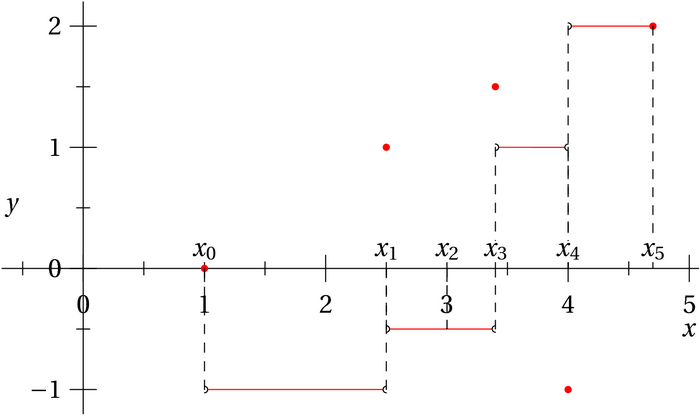
\includegraphics[width=5cm]{escalier1.png}.\\
L'ensemble des fonctions en escalier sur $[a,b]$ est un sous-espace vectoriel de l'espace vectoriel $\mathcal{F}([a,b],\mathbb{K})$.
\end{Definition}

\begin{Definition}[Riemnan intégrable] Une fonction $f$ définie sur $[a,b]$ est Riemnan intégrable si il existe une suite de fonctions en escalier convergeant uniformément vers $f$. Dans ce cas, on définit l'intégrale de $f$ par :
$$ \int_a^b f(t)dt\underset{\text{par définition}}{=}\lim_{n\to\infty}\int_a^b f_n(t)dt$$
\end{Definition}
%\Para{Remarque} La définition est justifiée car deux suites en escalier convergeant uniformément vers la fonction $f$ ont la même limite de leur intégrale.  En imposant uniquement la convergence simple, ce n'est pas le cas. Par exemple, les suites $f_n)$ et $(g_n)$ définies par:
% $$ \forall n \in \mathbb{N}^* :  g_n=0 \text{ et } \Fonction{f_n}{[0,1]}{\mathbb{R}}{x}{\begin{cases}n &\text{ si } x\in [1/n,2/n]\\0&\text{ sinon }\end{cases}}$$
% convergent simplement vers la fonction nulle et pourtant $\lim_{n\to \infty}\int_0^1 f_n(t)dt=1\neq 0 = \lim_{n\to \infty} \int_0^1 g_n(t)dt$. 
%\Para{Théorème d'approximation} Soit $f$ une fonction continue sur $[a,b]$.\\
%Alors il existe une suite de fonctions en escalier  convergeant uniformément vers la fonction $f$.
%\Para{Corollaire}L'ensemble des fonctions continues sur $[a,b]$ sont  Riemnan intégrable.
%
%
%
%
%
\subsection{Polynomial}
%
\begin{Theoreme}[Approximation de Stone-Weierstrass]Soit $f$ une fonction continue sur $[a,b]$.\\
Alors il existe une suite de fonctions polynomiales convergeant uniformément vers la fonction $f$.
\end{Theoreme}
\begin{Definition}[Développement en série entière (voir le chapitre)]
 Une \defi{série entière} réelle est une série de fonctions de la forme $\sum a_{n}x^{n}$ 
où les coefficients $a_n$ forment une suite réelle. On dit qu'une fonction $f\in \mathcal{C}^\infty$ est développable en série entière en $0$ si il existe une série entière $\sum a_{n}x^{n}$ tel que $f:x\mapsto\sum a_{n}x^{n}$ au voisinage de $0$.  
\end{Definition}


\subsection{Trigonométrique}
\begin{Theoreme}[Approximation de Stone-Weierstrass]
Soit $f$ une fonction complexe, continue et 2$\pi$-périodique.\\
Alors il existe une suite de fonctions polynômes trigonométrique  convergeant uniformément vers la fonction $f$.
\end{Theoreme}
\begin{Theoreme}[Développement en séries trigonométriques]
Soit $f$ une fonction complexe, $\mathcal{C}^1$ et 2$\pi$-périodique. On définit la série 
de polynôme trigonométrique par:
$ P_n(x)=\sum _{k=-n}^{+n}  c_{k}(f) e^{ikx}$ avec $c_{k}(f)={\frac {1}{2\pi}}\int _{-\pi}^{\pi}f(t)e^{-ikx}\mathrm {d} t$, appelés coefficients de fourrier.\\
Alors $(P_n)_{n\in\N}$ converge uniformément vers $f$.
\end{Theoreme}
Une application est le calcul de $\zeta(2)$. Soit $f:x\mapsto 1-\frac{x^2}{\pi^2}$ sur $[-\pi,+\pi]$, $2\pi$-périodique. Après calculs des coefficients de fourrier, on obtient que:
$$\forall x\in [-\pi,+\pi] :f(x)=  1-\frac{x^2}{\pi^2}=\frac{2}{3}-\frac{4}{\pi^2} \sum _{n=1}^{+\infty}(-1)^n \frac{\cos nx}{n^2}.$$
Donc $f(\pi)=0=\frac{2}{3}-\frac{4}{\pi^2} \sum _{n=1}^{+\infty}\frac{1}{n^2}$, d'où $\zeta(2)=\sum _{n=1}^{+\infty}\frac{1}{n^2}=\frac{\pi^2}{6}$.
\end{document}
